% TEX TS-program  pdflatex añadir un signo de ! al inicio y un signo de igual
% TEX encoding  UTF-8 Unicode añadir un signo de ! al inicio  y un signo de igual

% This is a simple template for a LaTeX document using the "article" class.
% See "book", "report", "letter" for other types of document.

%%%%%%%%%%%%%%%%%%%%%%%%%%%%%%%%%%%%%
%
% Template para producir documentos "camera ready" para Anales de la AFA
% 
%  No se debería tener que modificar nada del siguiente preámbulo, donde están 
%  las customizaciones para adaptar la clase "article" a los Anales AFA.
%
%%%%%%%%%%%%%%%%%%%%%%%%%%%%%%%%%%%%%
\documentclass[10pt,twocolumn]{article} 

\usepackage[utf8]{inputenc} % set input encoding (not needed with XeLaTeX)
\usepackage[spanish]{babel}


%%% DIMENSIONES DE LA PÁGINA
\usepackage{geometry} 
\geometry{a4paper} 
 \geometry{top=2.25cm} 
 \geometry{bottom=2.25cm} 
 \geometry{left=2.5cm} 
 \geometry{right=2cm} 


%%% PACKAGES
\usepackage{graphicx} 
\usepackage{paralist} % very flexible & customisable lists (eg. enumerate/itemize, etc.)
\usepackage{verbatim} % adds environment for commenting out blocks of text & for better verbatim
\usepackage{subfig} % make it possible to include more than one captioned figure/table in a single float
\usepackage{lipsum}  
\usepackage{hyperref}
\usepackage[superscript]{cite}  %REFERENCIAS EN SUPERÍNDICE

% Ajusta los captions de tablas y figuras a italics
\usepackage[format=plain,
            labelfont=it,
            textfont=it]{caption}
% These packages are all incorporated in the memoir class to one degree or another...

%%% HEADERS & FOOTERS
\usepackage{fancyhdr} % This should be set AFTER setting up the page geometry
\pagestyle{fancy} % options: empty , plain , fancy
\renewcommand{\headrulewidth}{0pt} % customise the layout...
\lhead{}\chead{}\rhead{}
\lfoot{}\cfoot{\thepage}\rfoot{}
%\renewcommand{\thefootnote}{\fnsymbol{footnote}}

\usepackage{varwidth}
\usepackage{authblk}
\newcommand{\filiacion}[2]{\affil[#1]{\protect\begin{varwidth}[t]{\linewidth}\protect\centering \normalfont#2 \protect\end{varwidth}}}
\newcommand{\autor}[2]{\author[#1]{\bf #2}}
\newcommand{\corresponding}[2]{\author[#1]{\bf #2\thanks{}}}
\newcommand\cauthemail[1]{\footnotetext{#1}}
\newcommand{\fecha}[1]{\date{\vspace{-1ex}\small{#1}}}
\newcommand{\titulo}[2]{\title{\bf{\large{#1 \\ \vspace{1.5ex} #2 }}}}
\newcommand{\esresumen}[1]{\small{#1 \par}\vspace{1.5ex}}
\newcommand{\pclaves}[1]{\small{\emph{#1} \par}\vspace{1.5ex}}
\newcommand{\enresumen}[1]{\small{#1 \par}\vspace{1.5ex}}
\newcommand{\keywords}[1]{\small{\emph{#1} \par}\vspace{1.5ex}}



%%% APARIENCIA DE TITULOS, SECCIONES Y SUBSECCIONES
\usepackage{sectsty}
\allsectionsfont{\fontsize{10}{12}\sffamily\bfseries\upshape} % (See the fntguide.pdf for font help)

\usepackage{titlesec}
\titlespacing*{\section}{0pt}{1.5ex}{0.8ex}
\titlespacing*{\subsection}{0pt}{1.2ex}{0.6ex}
\setcounter{secnumdepth}{1}   %no numera las subsecciones

\usepackage[nottoc,notlof,notlot]{tocbibind} % Put the bibliography in the ToC
\usepackage[titles,subfigure]{tocloft} % Alter the style of the Table of Contents
\renewcommand{\cftsecfont}{\rmfamily\mdseries\upshape}
\renewcommand{\cftsecpagefont}{\rmfamily\mdseries\upshape} % No bold!
\renewcommand\thesection{\Roman{section}}
\renewcommand\thesubsection{}



%%% PARA EL FORMATO DE TABLAS
\usepackage{booktabs} % for much better looking tables
\usepackage{array} % for better arrays (eg matrices) in maths
\makeatletter
\newcommand{\thickhline}{%
    \noalign {\ifnum 0=`}\fi \hrule height 1.5pt
    \futurelet \reserved@a \@xhline
}
\newcolumntype{"}{@{\hskip\tabcolsep\vrule width 1pt\hskip\tabcolsep}}
\makeatother
\newcolumntype{L}[1]{>{\raggedright\let\newline\\\arraybackslash\hspace{0pt}}m{#1}}
\newcolumntype{C}[1]{>{\centering\let\newline\\\arraybackslash\hspace{0pt}}m{#1}}
\newcolumntype{R}[1]{>{\raggedleft\let\newline\\\arraybackslash\hspace{0pt}}m{#1}}

\renewcommand\spanishtablename{Tabla}  

% Corresponding author
\usepackage[table,xcdraw]{xcolor}
\makeatletter
\renewcommand\@biblabel[1]{#1.}
\makeatother

\pagestyle{empty}

%%%%%% En principio no debería hacer falta modificar nada por encima de esta línea

%%%%%%%%%%%%%%%%%%%%%%%%%%%%%%%%%%%%%%%

%%% El contenido del documento comienza a partir de acá 

%título del trabajo: en el primer campo en castellano, en el segundo en inglés
\titulo{COMPARACIÓN DE TRES MÉTODOS DE DERIVACIÓN DE LA IRRADIANCIA SOLAR EFECTIVA PARA LA SÍNTESIS DE PRE-VITAMINA D\textsubscript{3} EN LA PIEL, EN LA CIUDAD DE ROSARIO, ARGENTINA}{COMPARISON OF THREE DERIVATION METHODS OF EFFECTIVE SOLAR IRRADIANCE FOR THE SYNTHESIS OF PRE-VITAMIN D\textsubscript{3} ON THE SKIN, IN ROSARIO, ARGENTINA}

\corresponding{1}{Adriana Ipiña}
\autor{2}{Montserrat Dávalos}
\autor{3}{Gamaliel López-Padilla}
\autor{1}{Rubén D. Piacentini}

%afiliaciones: se pueden combinar
\filiacion{1}{Instituto de Física Rosario (IFIR) – Universidad Nacional Rosario – Consejo Nacional de Investigaciones Científicas y
Técnicas, 27 de Febrero 210BIS – (S2000EKF) Rosario – Argentina.}
\filiacion{2}{Investigadora Independiente, (64810) México}
\filiacion{3}{Facultad de Ciencias Físico Matemáticas – Universidad Autónoma de Nuevo León, Pedro de Alba S/N - Ciudad
Universitaria San Nicolás de los Garza (66451) – Méxicoa.}

\fecha{Recibido: xx/xx/xx; Aceptado: xx/xx/xx} %No modificar


\setcounter{Maxaffil}{0}
\renewcommand\Affilfont{\itshape\small}


\begin{document}

\renewcommand{\abstractname}{}
\twocolumn[
  \begin{@twocolumnfalse}
    \maketitle
    \begin{abstract}\vspace{-12ex}
      \centering\begin{minipage}{\dimexpr\paperwidth-6cm}

        %Abstract en castellano
        \esresumen{En los últimos años, el interés por el estudio de la vitamina D ha aumentado debido al incremento en la incidencia de personas que presentan niveles deficientes de esta vitamina. Pocos alimentos la contienen de manera natural, siendo la principal fuente de obtención la radiación solar ultravioleta (UV), en la cual desencadena el mecanismo de la síntesis de la vitamina D en la parte superficial de la piel. En este estudio se determinó la irradiancia solar UV efectiva para la síntesis de pre-vitamina D\textsubscript{3} en la ciudad de Rosario, Argentina, utilizando tres métodos: a) Coeficiente de proporcionalidad, b) Ecuación de Herman y c) Modelo TUV. Los valores se compararon para condiciones de cielo despejado al mediodía solar. El cálculo de los tiempos de exposición solar (TES) se optimizó mediante un código python con el fin de obtener las dosis mínimas de radiación UV solar para sintetizar pre-vitamina D\textsubscript{3} mínima y para producir enrojecimiento de la piel debido a la dilatación de los vasos sanguíneos superficiales denominado eritema, diariamente en el periodo junio 2019 - mayo 2020. Se discute la variación de los TES para alcanzar una dosis mínima para la síntesis de pre-vitamina D\textsubscript{3} con una fotoexposición del 25\% de la superficie corporal (correspondiente a la cara, el cuello y los brazos). }
        \pclaves{Palabras Clave: radiación UV solar, vitamina D, dosis eritémica mínima, tiempos de exposición, Argentina.} %palabras clave

        %Abstract en inglés
        \enresumen{In the last years, interest in the study of vitamin D has raised due to the increase in the incidence of people with deficient levels of this vitamin. Few foods contain it naturally, being the main source of obtaining the ultraviolet solar radiation, which triggers the mechanism of the synthesis of vitamin D on the surface skin. In this study, the effective UV solar irradiance for the synthesis of pre-vitamin D\textsubscript{3} was determined in Rosario city, Argentina, using three methods: a) Coefficient of proportionality, b) Herman equation and c) TUV model. The values were compared in clear sky conditions at solar noon. The calculation of the solar exposure times (TES) was optimized by means of a python code in order to obtain the minimum doses for the synthesis of pre-vitamin D\textsubscript{3} and redness of the skin due to dilation of blood vessels also known as erythema, daily in the period june 2019 - may 2020. It is discussed the variation of the TES reaching the minimum dose of pre-vitamin D\textsubscript{3} with an photoexposure of 25\% of the body (face, neck and arms).}
        \keywords{Keywords: UV solar radiation, vitamin D, minimal erythemal dose, exposure times, Argentina.}  %key words

      \end{minipage}
      \vspace{4ex}
    \end{abstract}
  \end{@twocolumnfalse}
]
\thispagestyle{empty}

\setcounter{footnote}{1}
\cauthemail{ipina@ifir-conicet.gov.ar}  % Dirección de correo electrónico del corresponding author
\section{INTRODUCCIÓN}
La vitamina D participa en múltiples procesos en el  cuerpo humano, en varios otros mamíferos, reptiles y anfibios, interviene en la regulación de la homeostasis del calcio y por ende en el metabolismo óseo. La deficiencia de esta vitamina se asocia al incremento de algunos cánceres, enfermedades como el Parkinson, Alzheimer, entre otras.\cite{Zittermann2011,Afzal2013,KRAVIETZ201750} Pocos alimentos contienen esta vitamina de manera natural, siendo la radiación UV solar la principal fuente de síntesis en la piel expuesta. La radiación ultravioleta (UV) solar que llega a la superficie terrestre varía esencialmente en función de la composición atmosférica (especialmente O\textsubscript{3} estratosférico y troposférico), la ubicación geográfica, la hora del día y los días del año. El  intervalo de radiación UV es la más energética por fotón incidente (280-400 nm) y es la que desencadena las reacciones fotoquímicas importantes en la piel humana al interactuar con el 7-dehidrocolesterol (7-DHC) presente en las membranas plasmáticas de los queratinocitos de la epidermis y en los fibroblastos de la dermis.\cite{2002,brunser_radiacion_2005,Olds2008} Produciéndose dos tipos de vitamina D generada a partir de la interacción entre los fotones de radiación ultravioleta solar y la piel: la vitamina D\textsubscript{2} (ergocalciferol) sintetizada en los vegetales y la vitamina D\textsubscript{3} (colecalciferol) sintetizada en la piel humana.\cite{Zhang2010} Cuando el precursor 7-dehidrocolesterol presente en la piel, interactúa con fotones de radiación UV se convierte en pre-vitamina D\textsubscript{3}. Esta última se libera de la membrana celular y se asocia a su proteína transportador en sanguineo que es la $\alpha$1-globulina y viajando por el torrente sanguíneo llega al hígado en donde es hidroxilada, produciendo 1,25-hidroxivitamina D\textsubscript{3}, la forma activa de la vitamina D.\cite{brunser_radiacion_2005}

Por otro lado, la sobreexposición solar UV también puede producir efectos nocivos a largo plazo, que van desde el fotoenvejecimiento, fotodermatosis hasta cánceres de piel y cataratas.\cite{Gilaberte2011,Modenese2016} Por esta razón es de gran importancia poder determinar los tiempos óptimos de exposición solar para la síntesis la pre-vitamina D\textsubscript{3} sin provocar un daño a la piel (ej. eritema). Con este objetivo se utiliza la definición de la dosis efectiva de radiación solar:
\begin{equation}
  Dosis=\int_{t_1}^{t_2} \int_{200nm}^{400nm} E_\lambda\cdot S_\lambda d\lambda dt = \int_{t_1}^{t_2}E_tdt \,\, [J/m^2] \label{eq:dosis}
\end{equation}
donde E$_\lambda$ es la irradiancia solar espectral a nivel del suelo, S$_\lambda$ es el espectro de acción biológica de la síntesis de la pre-vitamina D\textsubscript{3} o eritémica (según sea el caso) y cuyo producto integrado sobre la longitud de onda representa la irradiancia efectiva, E\textsubscript{t}. Esta irradiancia de acuerdo a sus respectivos S$_\lambda$, definen las irradiancias de pre-vitamina D\textsubscript{3} (E\textsubscript{vitD}) y eritémica (E\textsubscript{er}).
La dosis mínima para mantener niveles adecuados de vitamina D\textsubscript{3} en una exposición de cuerpo completo es de 0.34 SDD (Dosis Estándar de vitamina D, SDD por sus siglas en inglés, equivalente a 100 J/m\textsuperscript{2} de exposición). Para una exposición del 25\% del cuerpo (brazos, cuello y cara) la dosis mínima es de 136 J/m\textsuperscript{2} y la dosis mínima para generar eritema en un fototipo de piel II es de 250 J/m\textsuperscript{2}, en la clasificación de Fitzpatrick.\cite{Fitzpatrick1988,UVDoses} Ambas dosis se consideran como valores de referencia en este trabajo para determinar los tiempos de exposición solar (TES). Se presenta la estimación de la irradiancia solar efectiva para la producción de la vitamina D\textsubscript{3}, comparando tres métodos: Coeficiente de proporcionalidad,\cite{UVDoses} Ecuación de Herman\cite{Herman2010} y Modelo TUV.\cite{Madronich1987} En particular, los resultados obtenidos con el modelo TUV se utilizaron para calcular los TES correspondientes a cada efecto biológico, en la ciudad de Rosario, Argentina.

\section{MATERIALES Y MÉTODOS}
Los datos de la columna total de ozono (O\textsubscript{3}) utilizados en este trabajo provienen de la Colección 3, OMTD3 v8.5, en Unidades Dobson (DU), medidos por el Instrumento de Monitoreo de Ozono (OMI) para las coordenadas de la ciudad de Rosario, Argentina. A bordo del satélite AURA-NASA, OMI realiza observaciones diarias en una superficie de 13x24 Km\textsuperscript{2} en el nadir \href{(disc.gsfc.nasa.gov)}{\url{disc.gsfc.nasa.gov}}. Por otro lado, se utilizó un espectroradiómetro Optronic-OL756 y la estación meteorológica DAVIS para mediciones in situ de E$_\lambda$ e índice UV, respectivamente. Ambos ubicados en el Instituto de Física Rosario (CONICET-UNR), en la ciudad de Rosario

\begin{figure}[ht]
  \centering
  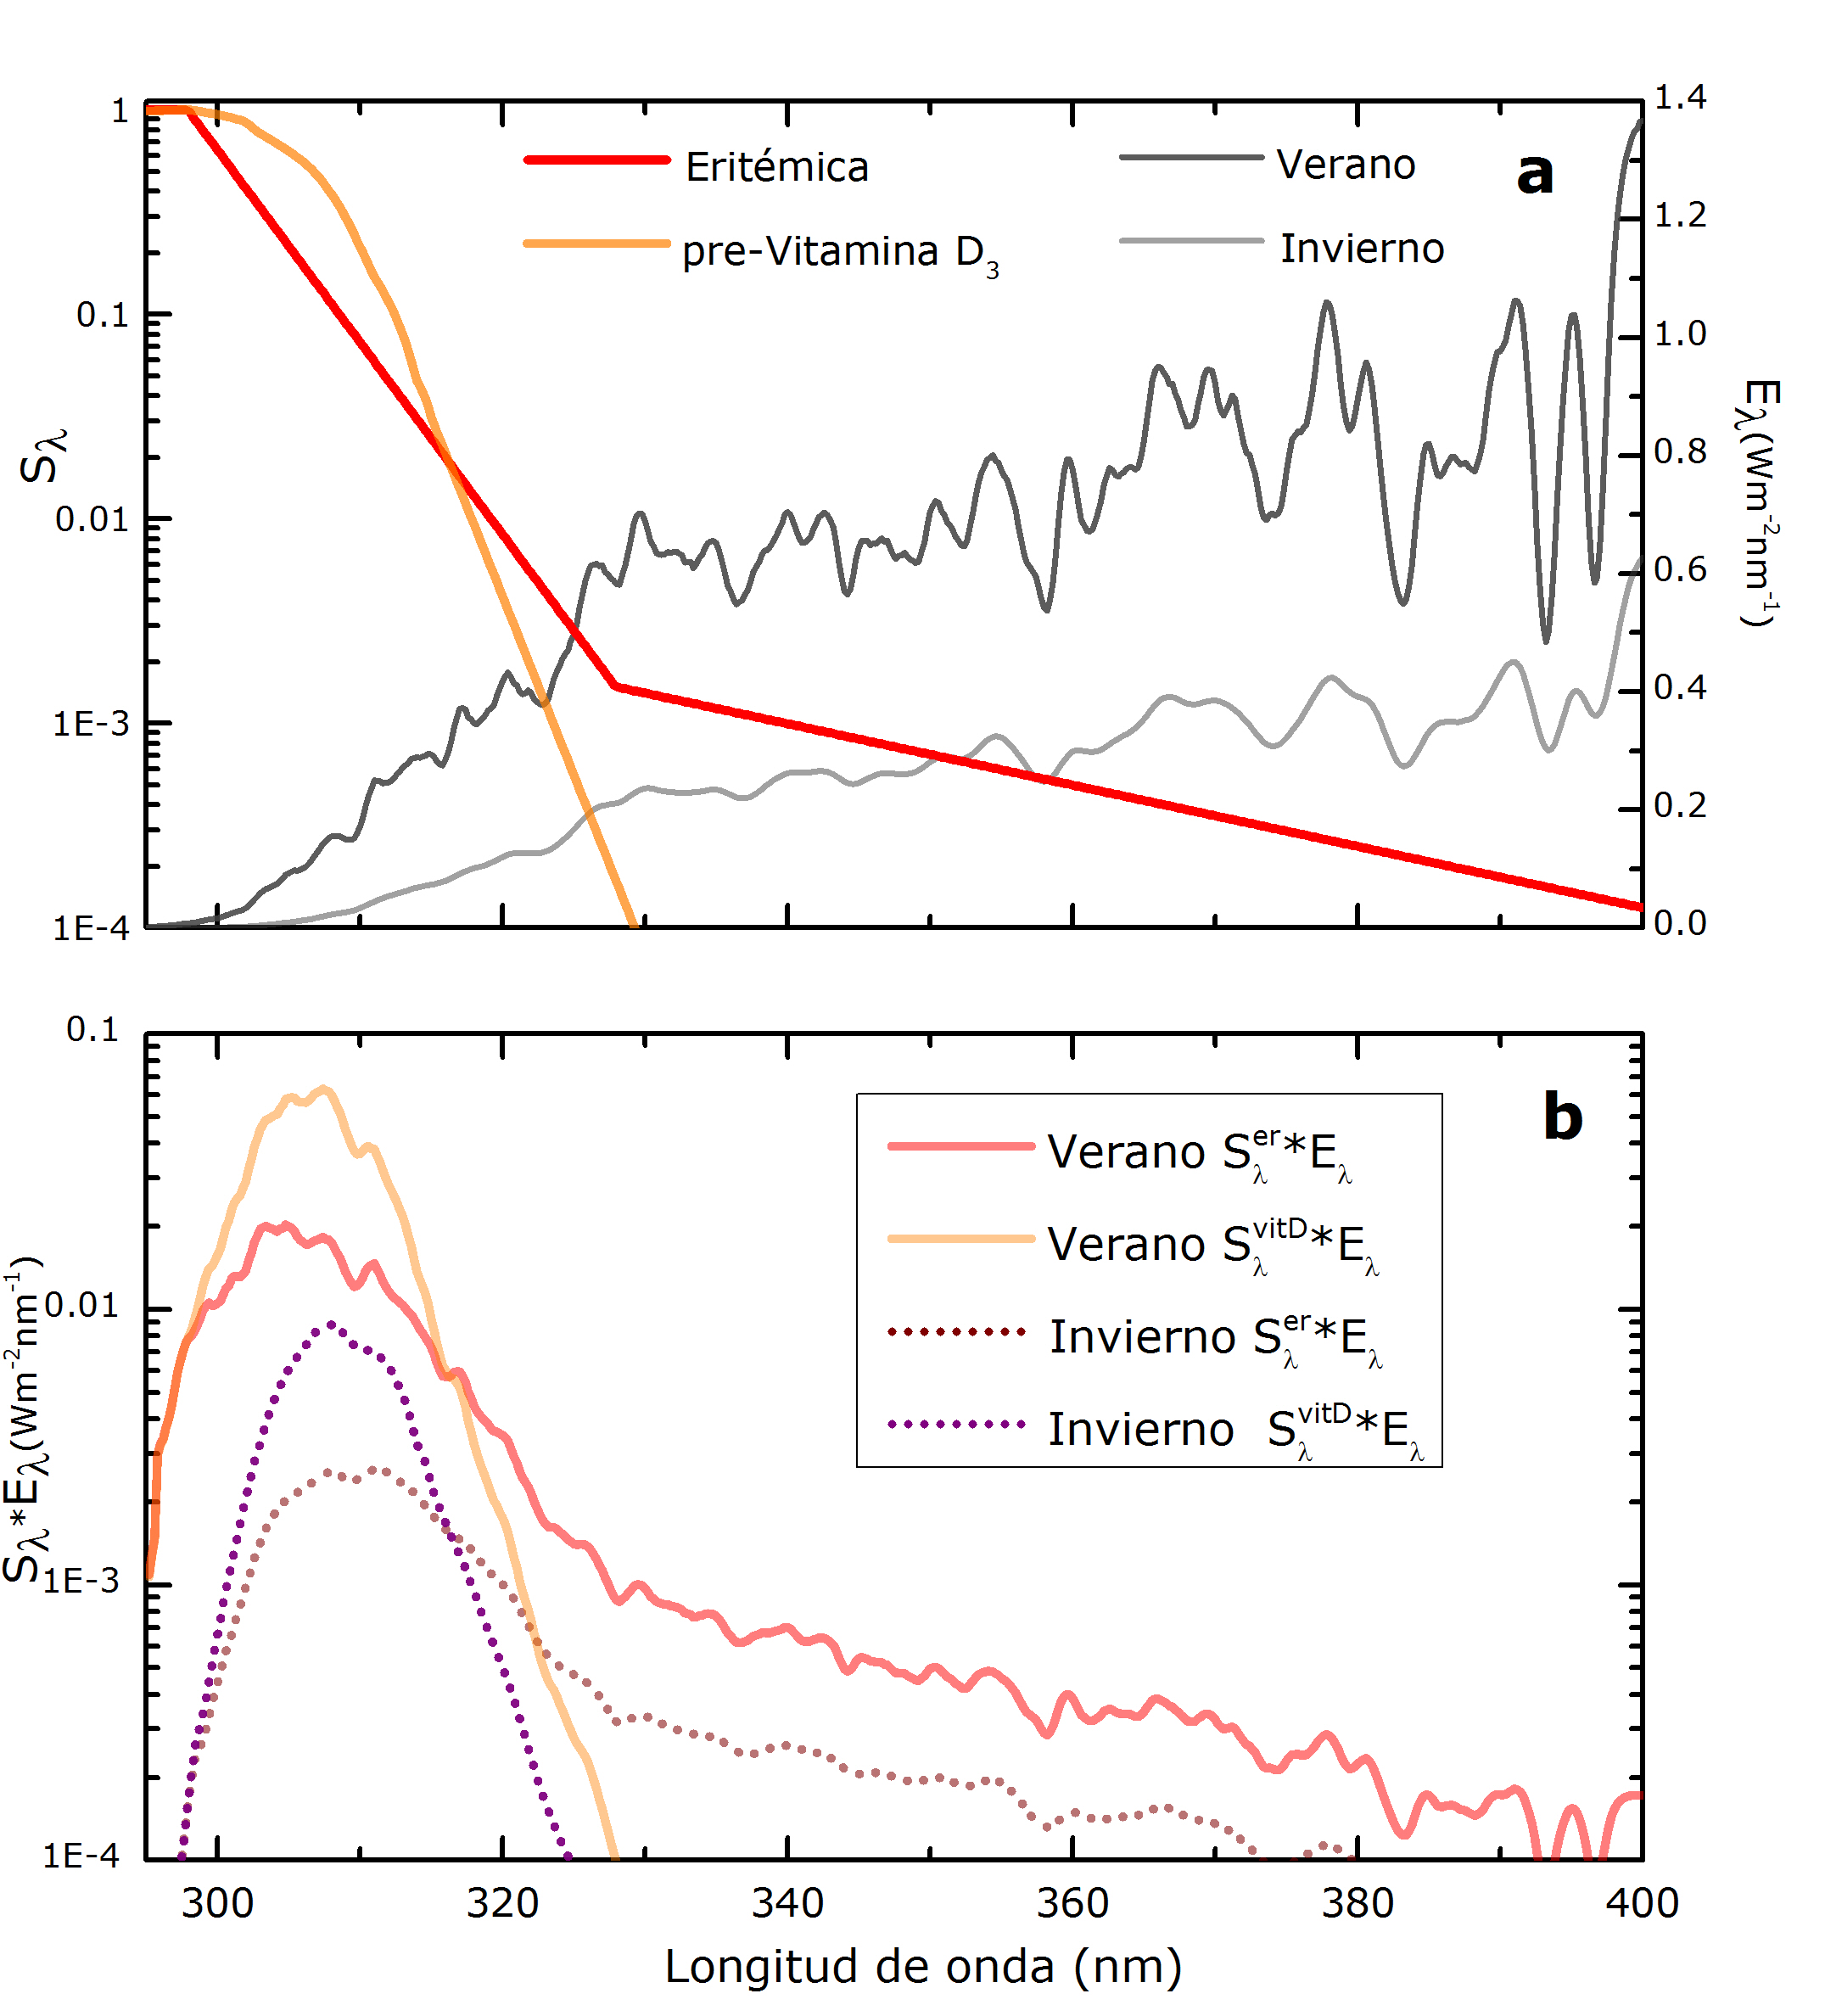
\includegraphics[scale=0.4]{factores.jpg}
  \caption{a)Espectros de acción de pre-vitamina D\textsubscript{3} y eritémica, e irradiancia espectral solar medida en cielo despejado, cerca de los solsticios de verano (28 de diciembre del 2011) e invierno (23 de junio del 2011), en la ciudad de Rosario. b) Irradiancia ponderada por cada espectro de acción y estación del año.}
  \label{fig:factores}
\end{figure}

\section{Coeficiente de proporcionalidad}
En el reporte de la Racionalización de la Nomenclatura de Dosis y Efectos de UV en Humanos\cite{UVDoses}, elaborado por la Commission Internationale de l’Eclairage (CIE) y la World Meteorological Organization (WMO), se define la relación:

\begin{equation}
  E_{vitD} = k \cdot E_{er}
  \label{ee:CIE}
\end{equation}
\begin{table*}[ht]
  \centering
  \caption{Coeficientes para obtener U y RAF en función del ángulo cenital solar $(\theta)= \frac{a+c\theta^2+e\theta^4}{1+b\theta^2+d\theta^4+f\theta^6}$ (Herman, 2010)\cite{Herman2010}}
  \label{table::parametros}
  \begin{tabular}{lll}
    \hline
      & \multicolumn{1}{c}{U}      & \multicolumn{1}{c}{RAF}     \\ \hline
    a & 0.9659616883022778         & 1.349378286522954           \\
    b & 0.0001089314449687077      & -0.0002926808443875372      \\
    c & -0.0002681987275053843     & -0.0003059282407232034      \\
    d & 1.410783665933483E$^{-8 }$ & 2.879164470755759E$^{-8}$   \\
    e & 1.894213900598701E$^{-8 }$ & 1.920553492457117E$^{-8}$   \\
    f & 1.695104643516458E$^{-12}$ & -8.580442654658103E$^{-13}$ \\ \hline
  \end{tabular}
\end{table*}

donde k toma dos valores distintos en verano e invierno para una ciudad del hemisferio sur. En este trabajo, los factores k para la ciudad de Rosario fueron determinados calculando las irradiancias E\textsubscript{er} y E\textsubscript{vitD}, por medio de Ec.\ref{eq:dosis} y las mediciones espectrales E$_\lambda$ realizadas bajo cielo despejado en verano e invierno (Figura \ref{fig:factores}). Posteriormente, las E\textsubscript{er} y E\textsubscript{vitD} fueron sustituidas en la Ec.\ref{ee:CIE}, obteniendo $k=1.6$ en invierno y de $k=2$ en verano. Luego de establecer los factores k para cada época del año fue posible estimar E\textsubscript{vitD} a partir de mediciones de irradiancia eritémica. El índice UV es una medida de la intensidad solar y el riesgo de sufrir eritema. Este índice es una cantidad adimensional que resulta de multiplicar la E\textsubscript{er} por 40 m$^2$/W y cuya escala va de 0 a 20 (o más). A partir de las mediciones diarias del índice UV al mediodía solar en cielo despejado de la estación DAVIS, fueron obtenidas las E\textsubscript{er} y finalmente por medio de la Ec.\ref{ee:CIE}, los valores de E\textsubscript{vitD}.

\section{Ecuación de Herman}
Herman\cite{Herman2010} determinó las E\textsubscript{vitD}D ejecutando el modelo TUV para diferentes ciudades alrededor del mundo. De los resultados derivó la siguiente ecuación general:
\begin{equation}
  E_{vitD}=U\left(\frac{O_3}{200}\right)^{-RAF}
  \label{eq:evitd}
\end{equation}
donde el O\textsubscript{3} es la columna total de ozono, RAF es el Factor de Amplificación de Radiación y U es una función de ajuste, estos dos últimos dependientes el ángulo cenital solar $(\theta)$. Esta ecuación permite determinar la E\textsubscript{vitD} sustituyendo el valor de O\textsubscript{3} medido en el sitio en cuestión y las funciones de RAF y U de acuerdo al ángulo cenital (relacionado a la hora del día). Los coeficientes para establecer U y RAF se muestran en la Tabla \ref{table::parametros}.

\section{Modelo TUV}
El modelo Tropospheric Ultraviolet Radiation (TUV) permite obtener los valores de radiación solar nanómetro a nanómetro mediante una ecuación de transferencia radiativa que lleva a determinar E$_\lambda$ a nivel del suelo, en los rangos ultravioleta, visible e infrarrojo cercano. El modelo incorpora el perfil de aerosoles cuya profundidad óptica (AOD) es de 0.23 a 340 nm (desde 5.24 km al espacio) y un perfil de O\textsubscript{3} correspondiente a la atmósfera estándar de EE. UU. Entre los datos de entrada más relevantes se encuentran las coordenadas geográficas del lugar, altura sobre el nivel del mar, AOD a 550 nm, reflectividad del suelo, albedo de dispersión simple, coeficiente de Angstrom, fecha y hora del día. La columna total de O\textsubscript{3} ingresada tiene un valor climatológico de acuerdo a la medición diaria de OMI.

Con el modelo TUV también se calcularon los valores de E\textsubscript{vitD} y E\textsubscript{er} para la latitud, longitud y altura sobre el nivel del mar (32.95°S, 60.62°W, 25 m s.n.m) de la ciudad de Rosario, Argentina. Las estimaciones se realizaron cada día, minuto a minuto entre las 11:00 - 15:00 h, en el periodo junio 2019 - mayo 2020. Posteriormente se seleccionaron las irradiancias al mediodía solar.

\section{Cálculo de los TES}
Por medio de un código en python y la Ec. \ref{eq:dosis} se calcularon los TES, utilizando las irradiancias E\textsubscript{vitD} y E\textsubscript{er} derivadas del modelo TUV. Se integraron las irradiancias en intervalos $t_2-t_1$ hasta alcanzar las dosis mínimas en fototipo II, necesarias para la producción de vitamina D\textsubscript{3} y para la aparición de eritema. Se consideró el comienzo de la exposición a las 11 h y se repitió la operación diariamente, revelando así el intervalo de tiempo $t_2-t_1$ para generar cada efecto a lo largo de un año.

\section{RESULTADOS}
La irradiancia pre-vitamina D\textsubscript{3} calculada al mediodía solar empleando los tres métodos se muestra en la Fig. \ref{fig:previtamin}. Como puede observarse, existe una razonablemente alta similitud entre los resultados obtenidos con la Ec. de Herman y con el modelo TUV. La diferencia relativa promedio fue de 5\% en verano y de 2\% en invierno, respecto al TUV. Mientras que las diferencias relativas en razón del Coeficiente de proporcionalidad con el TUV y la Ec. de Herman fueron de: 8.8\% y 8.4\% en invierno, así como de 22.3\% y 17.1\% en verano, respectivamente.

\begin{figure}[ht]
  \centering
  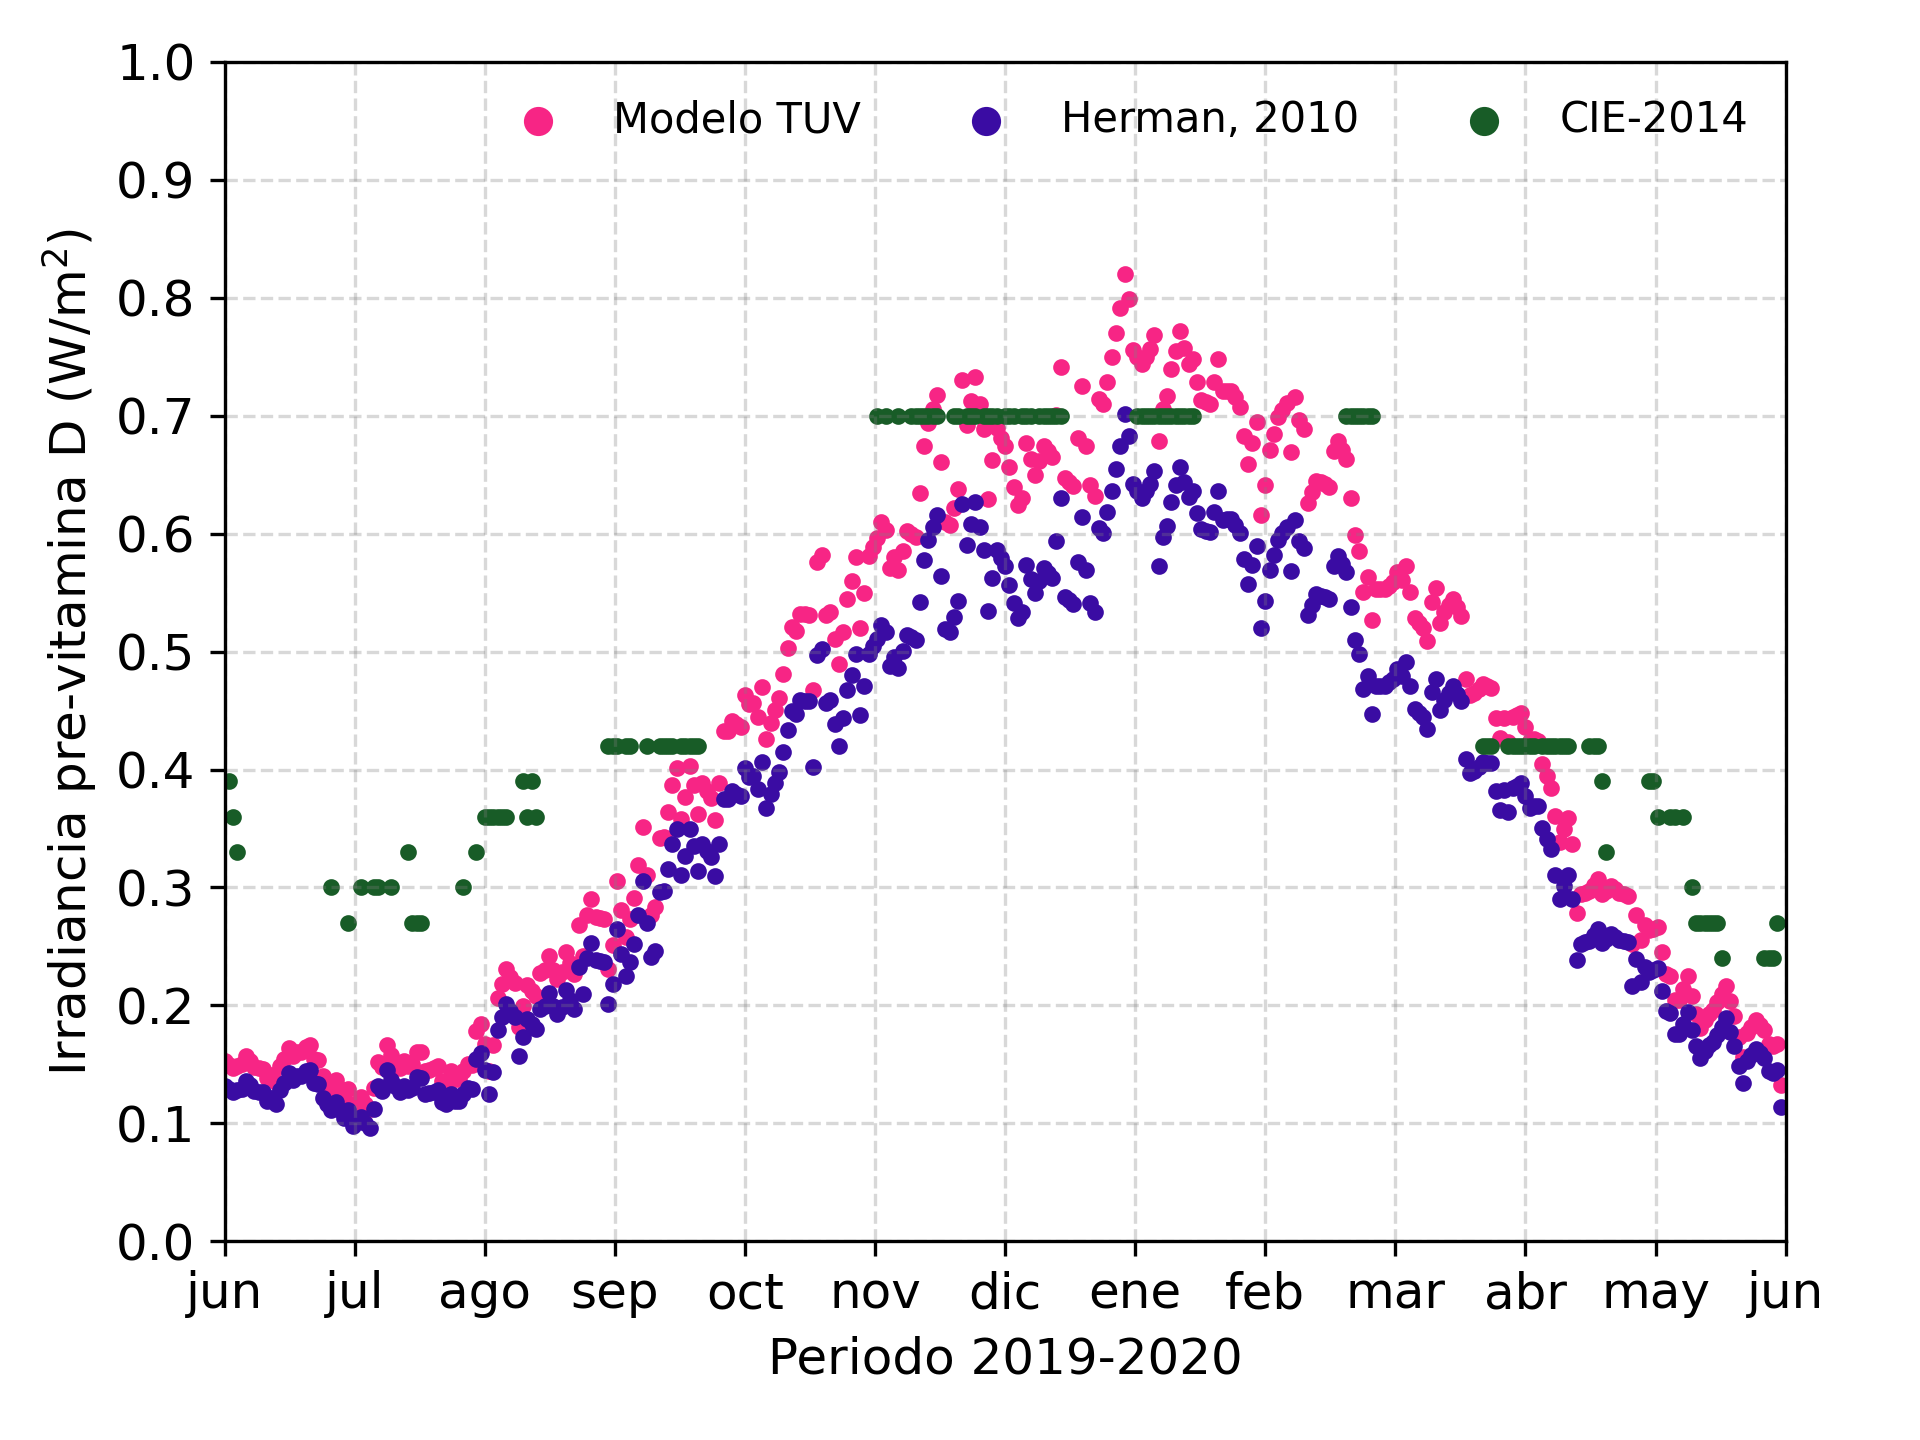
\includegraphics[scale=0.5]{Previtamin_D.png}
  \caption{Irradiancia de pre-vitamina D\textsubscript{3} para la ciudad de Rosario, obtenida con: Coeficiente de proporcionalidad, Ec. de Herman y Modelo TUV.}
  \label{fig:previtamin}
\end{figure}
\begin{table*}[ht]

  \centering\caption{TES obtenidos por Cabrera 2005\cite{cabrera_radiacion_2005}, Diaz et al. 2011\cite{Diaz2011} (gris) y análisis presente con modelo TUV (blanco): tasa de dosis (W/m$^2$), fototipo y dosis eritémica mencionada por cada autor.}
  \begin{tabular}{|c|c|c|c|c|c|c|c|c|}
    \hline
    Ciudad                     & \multicolumn{4}{c|}{\begin{tabular}[c]{@{}c@{}}Cabrera 2005\cite{cabrera_radiacion_2005}\\ (fototipo III, \\ Dosis 210 J/m$^2$)\end{tabular}} & \multicolumn{2}{c|}{\begin{tabular}[c]{@{}c@{}}Diaz et al. 2011\cite{Diaz2011}\\ (fototipo II, \\ Dosis=250 J/m$^2$)\end{tabular}} & \multicolumn{2}{c|}{\begin{tabular}[c]{@{}c@{}}Presente\\ (fototipo II, \\ Dosis=250 J/m$^2$)\end{tabular}}                                                                                                              \\ \cline{2-9}
                               & \multicolumn{2}{c|}{Tasa de dosis W/m$^2$}     & \multicolumn{6}{c|}{TES (minutos)}                                                                                                                                                                            \\ \cline{2-9}
                               & verano                                         & invierno                                       & verano                                          & invierno                    & verano                     & invierno                    & verano & invierno \\ \hline
    \begin{tabular}[c]{@{}c@{}}Santiago \\ de Chile\end{tabular} & \cellcolor[HTML]{DAD7D7}0.36                   & \cellcolor[HTML]{DAD7D7}0.06                   & \cellcolor[HTML]{DAD7D7}10                      & \cellcolor[HTML]{DAD7D7}56  & \cellcolor[HTML]{DAD7D7}21 & \cellcolor[HTML]{DAD7D7}119 & 16     & 43       \\ \hline
    Rosario                    & 0.29                                           & 0.1                                            & -                                               & -                           & -                          & -                           & 21     & 59       \\ \hline
    \begin{tabular}[c]{@{}c@{}}Punta\\ Arenas\end{tabular} & \cellcolor[HTML]{DAD7D7}0.13                   & \cellcolor[HTML]{DAD7D7}0.03                   & \cellcolor[HTML]{DAD7D7}26                      & \cellcolor[HTML]{DAD7D7}134 & \cellcolor[HTML]{DAD7D7}37 & \cellcolor[HTML]{DAD7D7}x   & 22     & x        \\ \hline
  \end{tabular}
  \label{table:TES}
\end{table*}
Un estudio\cite{LuChenHolick+2019+53+56} sobre el porcentaje de conversión de 7-DHC a pre-vitamina D\textsubscript{3} en diferentes latitudes, épocas del año y horas del día, reveló que a latitudes $>40^\circ$[S-N] en invierno, esta conversión es extremadamente ineficiente. La magnitud de este porcentaje resultó inversamente proporcional a la latitud en ciudades del continente americano. En el hemisferio norte, las ciudades de Boston y Edmonton tuvieron su máximo \% de conversión a pre-vitamina D\textsubscript{3} alrededor del mediodía solar el mes de junio, mientras que en el hemisferio sur, Buenos Aires y Ushuaia lo tienen el mes de diciembre. Estos resultados concuerdan con los obtenidos con los tres métodos de derivación de la irradiancia efectiva de pre-vitamina D\textsubscript{3} en Rosario, ya que el máximo valor se encontró en el mes de diciembre (Figura \ref{fig:previtamin}).

Para una exposición que comienza a las 11 h, en el periodo junio 2019 - mayo 2020 se estimaron los TES a partir de los resultados obtenidos con el modelo TUV (Fig. \ref{fig:TES}). En invierno los TES para comenzar la síntesis de pre-vitamina D\textsubscript{3} en personas con fototipo II, se encuentran en promedio a los 22$\pm$8 minutos y para la aparición de eritema a los 59$\pm$17 minutos. En verano, en promedio se requieren 6$\pm$1 minutos para alcanzar la dosis mínima de pre-vitamina D\textsubscript{3} y 21$\pm$3 minutos para la eritémica.

\begin{figure}[ht]
  \centering
  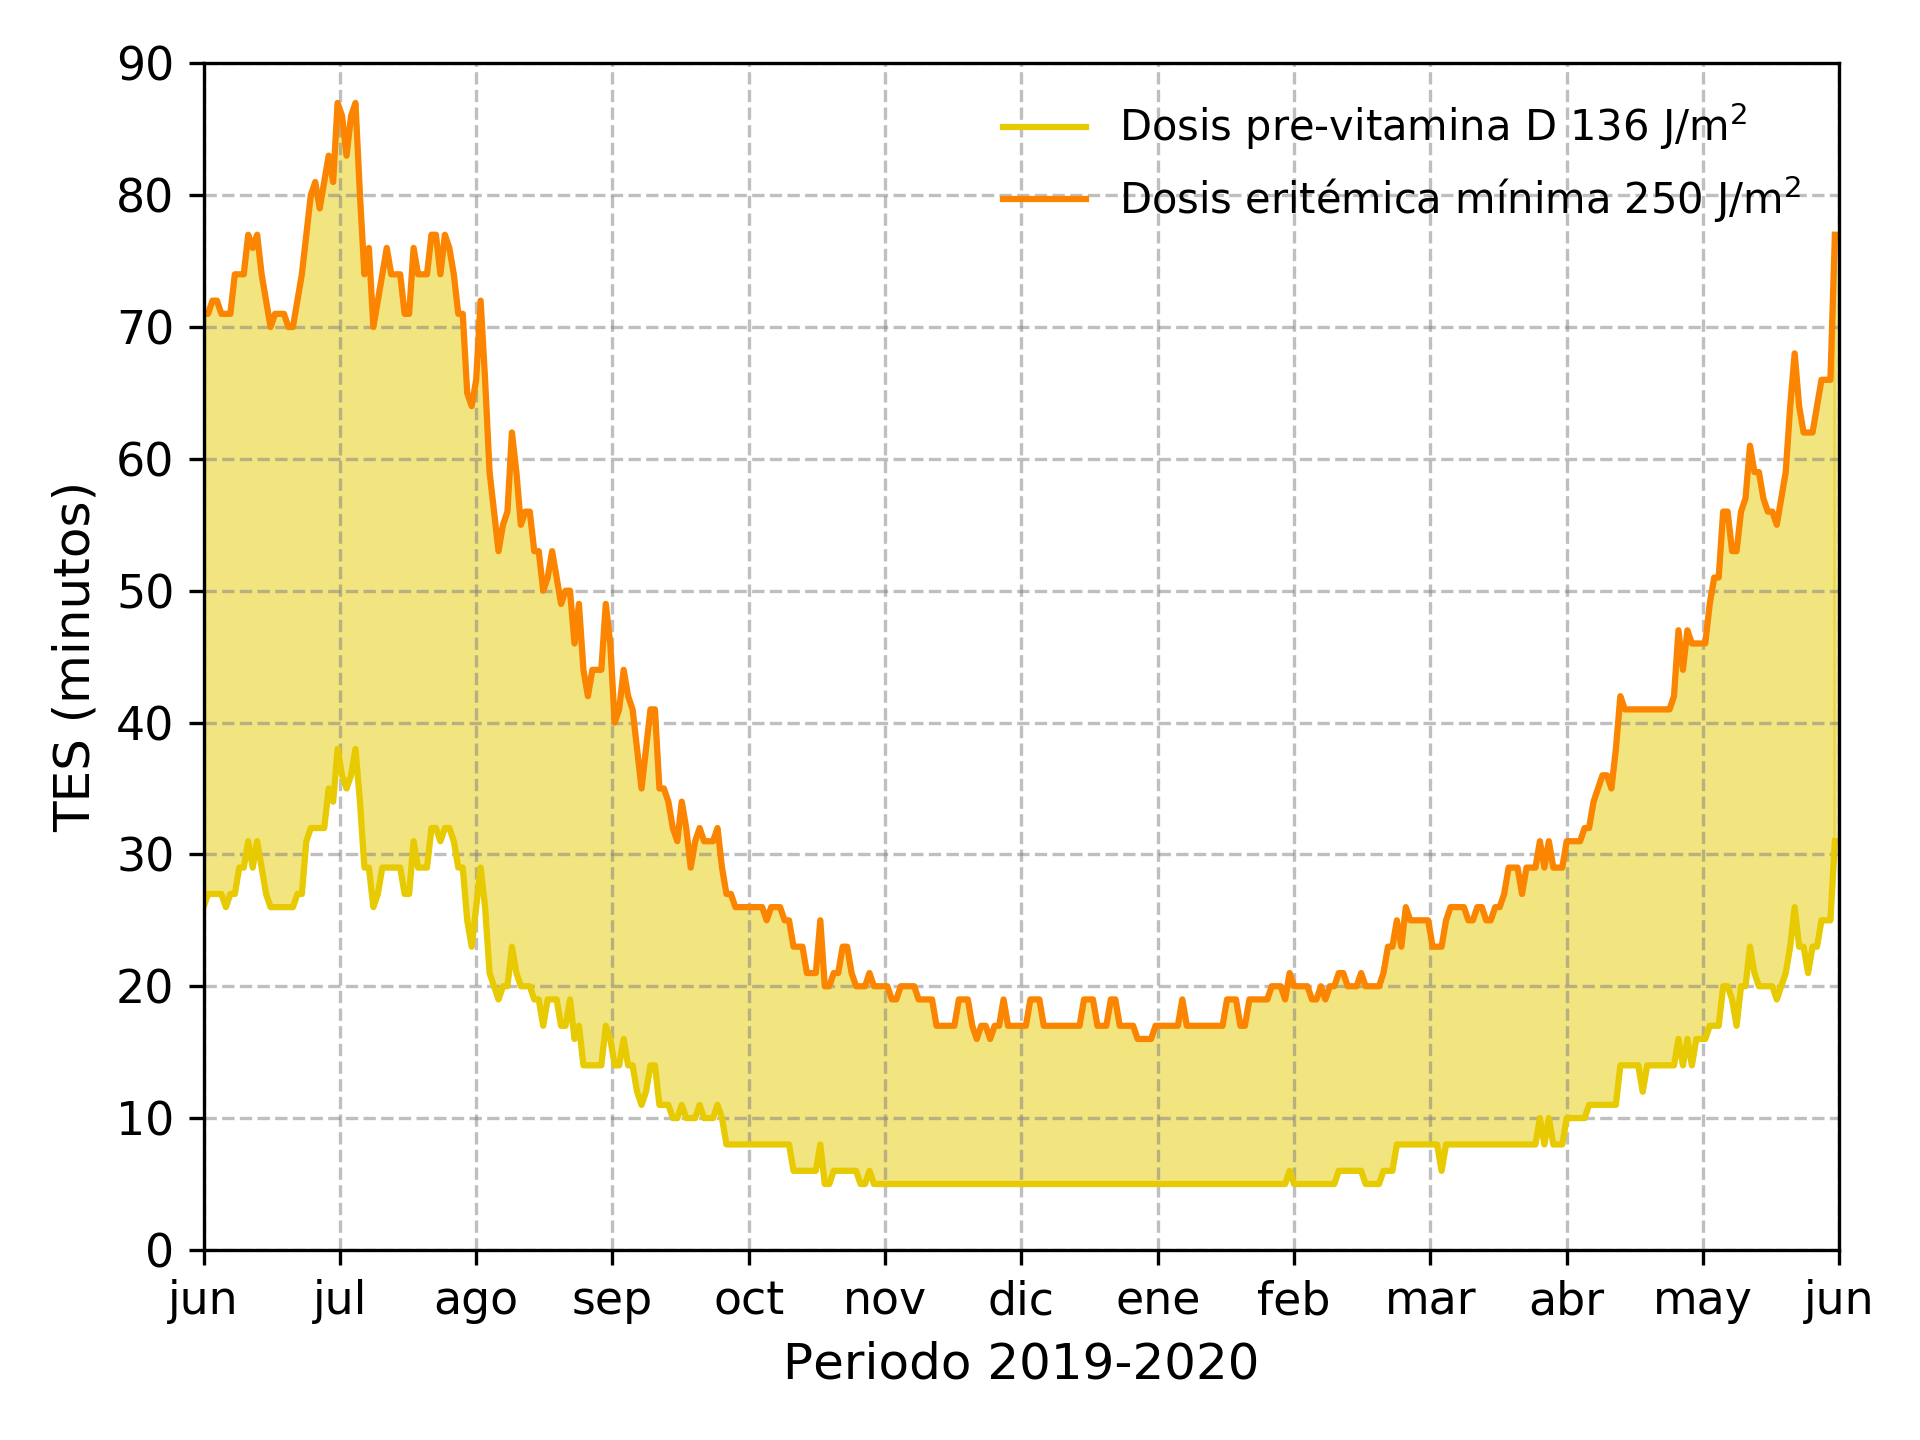
\includegraphics[scale=0.5]{dosis_vitamin.png}
  \caption{TES diarios para generar pre-vitamina D\textsubscript{3} (área amarilla) y límite para evitar el eritema de la piel en una persona de un fototipo de piel II (curva naranja). TES comenzando a las 11 h con cielo despejado, en la ciudad de Rosario.}
  \label{fig:TES}
\end{figure}

\section{DISCUSIÓN Y CONCLUSIONES}
El modelo TUV y la Ec. de Herman mostraron valores semejantes de irradiancia pre-vitamina D\textsubscript{3} debido a que ambos métodos consideran el D\textsubscript{3} y el $\theta$ como principales elementos de influencia. Además, particularmente en la ciudad de Rosario, las concentraciones de SO\textsubscript{2} y NO\textsubscript{2} no varían significativamente a lo largo del año. Sin embargo, los aerosoles pudieran tener una importante contribución en la atenuación del UV entre mayo-agosto cuando suelen tener lugar incendios en el delta del río Paraná frente a Rosario.\cite{Madronich1987} Respecto al método basado en el Coeficiente de proporcionalidad, aunque su aplicación resulta más simple, la precisión depende de los valores de k para cada época del año. En verano, este último subestima la magnitud de la irradiancia pre-vitamina D\textsubscript{3} con respecto a los otros dos métodos.

Diaz et al. 2011\cite{Diaz2011} calculó los TES para las dosis de síntesis de pre-vitamina D\textsubscript{3} y eritémica en un fototipo II, en una exposición del 9\% del cuerpo. Los TES para la síntesis de vitamina D\textsubscript{3} en Buenos Aires (a 300 km de Rosario) y Santiago de Chile, fueron de 13 y 12 minutos en verano, respectivamente.\cite{IPINA2012966} Estos TES para alcanzar la dosis mínima de pre-vitamina D\textsubscript{3} difieren más del doble respecto a la estimación hecha para la ciudad de Rosario (6±1 min). A pesar de que estas ciudades se encuentran a latitudes cercanas, en los primeros dos casos, los TES son más largos debido a que las mediciones no discriminan las condiciones de cielo y consideran un área expuesta del cuerpo de menor tamaño.

Un análisis comparativo de los TES para acumular la dosis mínima eritémica a diferentes latitudes fue realizado utilizando dos ciudades incluidas en los trabajos de Diaz et al. 2011\cite{Diaz2011} y Cabrera 2005\cite{cabrera_radiacion_2005}.  En la Tabla \ref{table:TES} se muestra para la ciudad de Santiago y de Punta Arenas, las tasas de dosis medidas y los TES de acuerdo a los fototipos y dosis consideradas. Los valores para la ciudad de Rosario corresponden a los valores estimados para este trabajo con el Modelo TUV, incorporando la aproximación también para las otras ciudades.

Los valores para Santiago de Chile estimados con el modelo TUV, se encuentran entre los otros dos TES de referencia. Las diferencias se pueden atribuir muy probablemente a la nubosidad, hora del día y número de mediciones, así como diferencias entre los parámetros de entrada introducidos en el modelo. Para Punta Arenas, los TES en los tres estudios muestran concordancia en verano sin embargo, en invierno la dosis no es alcanzada con los resultados de irradiancia eritémica del modelo TUV al igual que lo reportó Diaz et al. 2011\cite{Diaz2011}. Para alcanzar la dosis mínima eritémica en Rosario se necesita en promedio TES de 21$\pm$3 min en verano, los cuales se encuentran en el rango esperado de acuerdo a la latitud.

El modelo TUV, la Ec. de Herman y el Coeficiente de proporcionalidad estiman valores para cielo despejado, en consecuencia podrían ser considerados como un límite superior para la exposición a la radiación solar UV a lo largo del año. Este estudio podría extenderse en un futuro para analizar la contribución de las nubes y los aerosoles,\cite{Kim2020} así como la mezcla en altura con la capa límite atmosférica.
\section{REFERENCIAS}
\bibliographystyle{abbrv} %orden alfabético 
%\bibliographystyle{aichej} %orden de mención
\renewcommand{\refname}{}
\bibliography{references}
\end{document}